\section{Physical Design}

The idea behind the physical design is to show how the programs works
on a physical (hardware) level. This means storage space, hardware
requirements, and such. Because The OS reqs are already discussed
previously, this means that it will not be touched upon again. This
section will show visuals demonstrating how the various pieces of the
application connect together.

\subsection{Database Operations}

As stated previously, there is a database managed through SQLite
which is used for handling data processing. This is the central piece
to the programs operations, seen in Figure \ref{fig:DBOperations}.

\begin{figure}[htb]
	\centering
	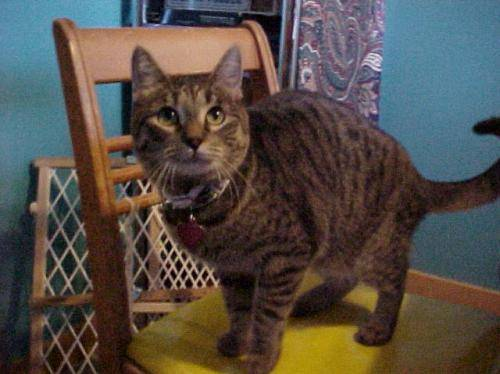
\includegraphics[width=10cm]{./Images/cats_00001.jpg}
	\caption{Database Operations}
	\label{fig:DBOperations}
\end{figure}

The overall structure adds new files to the file system, as seen
previously in section \ref{subsec:Installation}. These folders aren't
explicitly talked about, but that's what I'm going to do now.

\subsection{Logging}

Essentially, the logs directory will hold all logs of the
application. Every time the application is run, a new log file is
created with the program name, version, and current time. The goal is
to be able to identify what went wrong and how to replicate it should
any issues arise. The log file may be filled with lots of lines, but
the overall size should remain small. These log files are not read by
the program at all, only written to. In fact, the program only checks
for the existence of the logs directory.

\begin{figure}[htb]
	\centering
	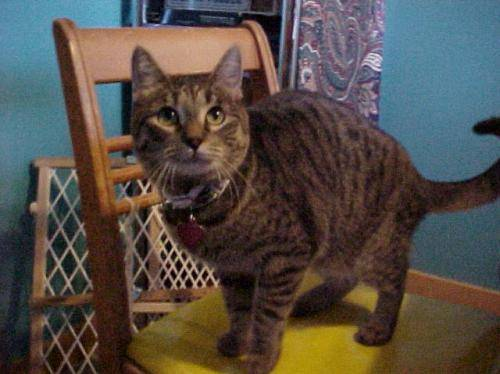
\includegraphics[width=10cm]{./Images/cats_00001.jpg}
	\caption{Program only writes to logs directory}
	\label{fig:DBOperations}
\end{figure}

\subsection{Themes}

The themes directory holds all the themes as YAML files. The goal was
to find a cross-section between easy to read from, and easy for users
to write. YAML files do exactly that.

The program looks at the current folder and checks to see if the
themes directory exists. If it doesn't, then the program creates it and
inserts the Light and Dark themes. If the themes folder does exist,
the program checks for the existence of the Light and Dark themes and creates
them if they do not exist.

The user is capable of modifying these themes, since they are not
checked explicitly to make sure they match the defaults, but I highly
advise against it. Should there be any bugs or changes to the
program in regard to the Light or Dark themes, I cannot guarantee proper
functionality. The intended usage was to copy the structure of the
given files into a new file and change the values for the name and colors.

\begin{figure}[htb]
	\centering
	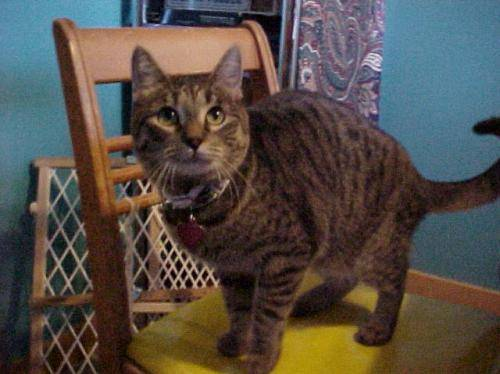
\includegraphics[width=10cm]{./Images/cats_00001.jpg}
	\caption{Theme Reading/Writing}
	\label{fig:DBOperations}
\end{figure}

\subsection{Imports}

To import data from files, there are three options:
\begin{enumerate}
	\item CSV
	\item SQL
	\item TXT
\end{enumerate}

In each case, the user is prompted to select the file from their file
system that has a matching filetype. The file is assumed to work and
be compatible. If not, then the program most likely crashes.

\begin{figure}[htb]
	\centering
	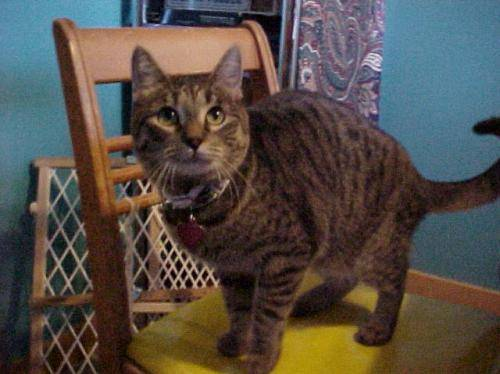
\includegraphics[width=10cm]{./Images/cats_00001.jpg}
	\caption{Importing photo}
	\label{fig:DBOperations}
\end{figure}

\subsection{Exports}

To export data into files, there are three options:
\begin{enumerate}
	\item CSV
	\item SQL
	\item Markdown
\end{enumerate}

In each case, the user is prompted to select a directory from the
file system to store the file to be created, and then also write the
name of the file to be saved as. Should the user write an extension,
the program will remove it and overwrite it with the
specified extension.

\begin{figure}[htb]
	\centering
	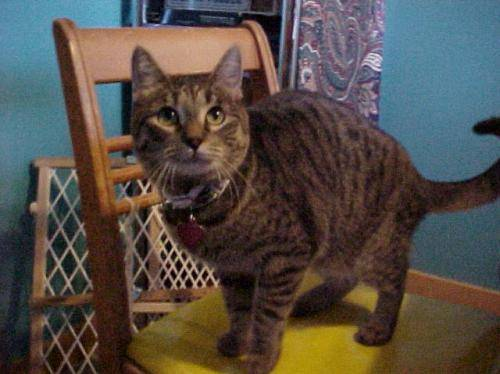
\includegraphics[width=10cm]{./Images/cats_00001.jpg}
	\caption{Exporting photo}
	\label{fig:DBOperations}
\end{figure}
